\documentclass[letterpaper,12pt]{article}
\usepackage[brazil,english,portuguese]{babel}
\usepackage[T1]{fontenc}
\usepackage[numbers]{natbib}
\usepackage{ae}
\usepackage[utf8]{inputenc}
\usepackage[dvipsnames]{color}
\usepackage{graphicx}
\usepackage{epsfig}
\usepackage{float}
\usepackage{multirow}
\usepackage{amssymb, amsmath, amsfonts}
\usepackage{setspace}

\topmargin		0 cm
\hoffset		0 cm
\voffset		0 cm
\evensidemargin		0 cm
\oddsidemargin		0 cm
\setlength{\textwidth}{16 cm}
\setlength{\textheight}{21 cm}
\onehalfspacing

\newcommand{\titulo}{
\iflanguage{portuguese}{ Controle Dinâmico da Inviabilidade para Programação Não Linear}
{ Dynamic Control of Infeasibility for Nonlinear Programming }
}
\newcommand{\autor}{Abel Soares Siqueira}
\newcommand{\orientador}{Francisco A. M. Gomes}

\numberwithin{equation}{section}

% \newcommand{\visiblelbl}[1]{\label{#1}{\color{red}{#1}}}
\newcommand{\visiblelbl}[1]{\label{#1}}
\newcommand{\meio}{\frac{1}{2}}
\newcommand{\Meio}{\dfrac{1}{2}}
\newcommand{\norma}[1]{\left\Vert{#1}\right\Vert}
\newcommand{\modulo}[1]{\left\vert{#1}\right\vert}
\renewcommand{\emph}[1]{{\bf #1}}
\newcommand{\No}{N$^\circ$}
\newcommand{\rhomax}{\rho_{\max}}
\newcommand{\R}{\mathbb{R}}
\newcommand{\Rn}[1]{\mathbb{R}^{#1}}
\newcommand{\vetor}[2]{\left[\begin{array}{c} {#1}\\{#2} \end{array}\right]}
\newcommand{\bigo}{\mathcal{O}}

\begin{document}
\selectlanguage{portuguese}
\begin{center}
  \Large \bf \titulo
\end{center}
\begin{center}
  \autor \\
  Supervisor: \orientador
\end{center}
\begin{abstract}
\iflanguage{portuguese}{
O método de Controle Dinâmico da Inviabilidade,
recentemente estendido no doutorado em progresso de Abel Soares Siqueira
para incluir restrições de desigualdade, mostrou-se um competidor
promissor entre os métodos para programação não linear.
A implementação do novo método, denominada \emph{DCICPP}, foi
comparada com o método IPOPT 
e obteve um bom desempenho.
O DCICPP já consegue encontrar eficientemente a solu\c{c}\~{a}o
de 698 problemas do CUTEr em 2 horas.
Neste projeto
pretendemos estudar maneiras de aumentar ainda mais a
robustez do {DCICPP}, avaliando
outras estratégias para resolver os subproblemas.
Tamb\'{e}m queremos melhorar aspectos pr\'{a}ticos do algoritmo,
por exemplo,
implementar uma maneira
de lidar com as variáveis fixas no problema e avaliar possibilidades de
lidar com Jacobianas mal condicionadas.
Esse projeto é uma extensão da tese de doutorado de Abel Soares Siqueira, 
da Matemática Aplicada, pelo IMECC, com previsão de defesa para Novembro de
2013, e está vinculado ao projeto temático 2013/05475-7.
}
{
The Dynamic Control of Infeasibility method, recently expanded in the Ph.D.
in progress of Abel Soares Siqueira to include inequality constraints, proved to
be a good choice amongst the methods for nonlinear programming. The method's
implementation, called DCICPP, was compared to the IPOPT method and
achieve
a good performance. The DCICPP method can already find efficiently the solution
of 698 problem of CUTEr in 2 hours.
In this project, we intend to study ways of increasing even more the strength of
the DCICPP method, considering other strategies to solve the subproblems. We also
want to improve the practical aspects of the algorithm, for instance,
accepting fixed variables in the problem, and pondering
possibilities to handle ill-conditioned Jacobian matrices.
This project is an extension of the Ph.D. of Abel Soares Siqueira, in Applied
Mathematics, from the IMECC, with
defense
expected in November, 2013, and is tied to the thematic projetc 2013/05475-7.
}

\vspace{1 cm}
{\noindent\bf Keywords:} Nonlinear Programming, Constrained Opmitization,
Composite-step Methods.}
\end{abstract}

\newpage
\selectlanguage{english}
\begin{center}
  \Large \bf \titulo
\end{center}
\begin{center}
  \autor \\
  Supervisor: \orientador
\end{center}
\begin{abstract}
\iflanguage{portuguese}{
O método de Controle Dinâmico da Inviabilidade,
recentemente estendido no doutorado em progresso de Abel Soares Siqueira
para incluir restrições de desigualdade, mostrou-se um competidor
promissor entre os métodos para programação não linear.
A implementação do novo método, denominada \emph{DCICPP}, foi
comparada com o método IPOPT 
e obteve um bom desempenho.
O DCICPP já consegue encontrar eficientemente a solu\c{c}\~{a}o
de 698 problemas do CUTEr em 2 horas.
Neste projeto
pretendemos estudar maneiras de aumentar ainda mais a
robustez do {DCICPP}, avaliando
outras estratégias para resolver os subproblemas.
Tamb\'{e}m queremos melhorar aspectos pr\'{a}ticos do algoritmo,
por exemplo,
implementar uma maneira
de lidar com as variáveis fixas no problema e avaliar possibilidades de
lidar com Jacobianas mal condicionadas.
Esse projeto é uma extensão da tese de doutorado de Abel Soares Siqueira, 
da Matemática Aplicada, pelo IMECC, com previsão de defesa para Novembro de
2013, e está vinculado ao projeto temático 2013/05475-7.
}
{
The Dynamic Control of Infeasibility method, recently expanded in the Ph.D.
in progress of Abel Soares Siqueira to include inequality constraints, proved to
be a good choice amongst the methods for nonlinear programming. The method's
implementation, called DCICPP, was compared to the IPOPT method and
achieve
a good performance. The DCICPP method can already find efficiently the solution
of 698 problem of CUTEr in 2 hours.
In this project, we intend to study ways of increasing even more the strength of
the DCICPP method, considering other strategies to solve the subproblems. We also
want to improve the practical aspects of the algorithm, for instance,
accepting fixed variables in the problem, and pondering
possibilities to handle ill-conditioned Jacobian matrices.
This project is an extension of the Ph.D. of Abel Soares Siqueira, in Applied
Mathematics, from the IMECC, with
defense
expected in November, 2013, and is tied to the thematic projetc 2013/05475-7.
}

\vspace{1 cm}
{\noindent\bf Keywords:} Nonlinear Programming, Constrained Opmitization,
Composite-step Methods.}
\end{abstract}

\newpage
\section{Introdução}

Muitos m\'{e}todos desenvolvidos para resolver o problema de programa\c{c}\~{a}o
n\~{a}o-linear s\~{a}o baseados na ideia de passos compostos. Em geral, um
tipo de passo, chamado de passo normal, investe na factibilidade primal 
enquanto o outro, chamado de passo tangente, na 
factibilidade dual. Os trabalhos \cite{bib:biegler,bib:byrd_gilbert,bib:byrd_hribar,bib:dennis,bib:el_alem,bib:gomes,bib:lalee} tamb\'{e}m seguem essa linha.
Nesse tipo de m\'{e}todo \'{e} necess\'{a}rio
alguma maneira de limitar o tamanho ou aceita\c{c}\~{a}o desses passos, 
para que o objetivo de um
n\~{a}o destrua o resultado do outro. Uma estrat\'{e}gia utilizada tradicionalmente
\'{e} a de fun\c{c}\~{a}o de m\'{e}rito, onde uma fun\c{c}\~{a}o \'{e} criada
utilizando uma combina\c{c}\~{a}o 
da fun\c{c}\~{a}o objetivo e de alguma
penaliza\c{c}\~{a}o sobre o valor das restri\c{c}\~{o}es. 

O método de Controle Dinâmico da Inviabilidade proposto por
\citet*{bib:chico} define uma nova estrat\'{e}gia para a aceita\c{c}\~{a}o
dos passos. Essa estrat\'{e}gia, chamada de Cilindros de Confian\c{c}a,
permite que os passos 
tangentes tenham grande magnitude longe da solução, 
e tamb\'{e}m permitem fazer mais de um passo
normal para encontrar um ponto suficientemente pr\'{o}ximo
ao conjunto fact\'{i}vel. Esse método, originalmente proposto para problemas 
de igualdade, foi estendido para problemas gerais de programação não linear
na tese de Abel Soares Siqueira, permitindo que o problema também tenha 
restrições não lineares de desigualdade e limitantes para as variáveis.

\section{Motivação e Objetivos}

Considere o problema de programa\c{c}\~{a}o n\~{a}o linear na forma
\begin{equation*}
 \begin{array}{rrrrcll}
  \min & f(x) \\
  \mbox{suj. a} &     &      & c_E(x) &   =  & 0, \\
  & c_L & \leq & c_I(x) & \leq & c_U, \\
  & b_L & \leq &      x & \leq & b_U, \\
  \end{array}
\end{equation*}
onde $f:\Rn{n}\rightarrow\R, c_E:\Rn{n}\rightarrow\Rn{m_E},
c_I:\Rn{n}\rightarrow\Rn{m_I} \in \mathcal{C}^2$, $c_L, c_U \in \Rn{m_I}$ e
$b_L, b_U \in \Rn{n}$.
Essa forma \'{e} a considerada pelo repositório CUTEr (\cite{bib:cuter}) 
A partir desse problema, criamos o problema de igualdade e caixas
\begin{equation*}
 \begin{array}{rrrrcll}
  \min & f(x) \\
  \mbox{suj. a} 
&     &      & c_E(x) &   =  & 0, \\
&     &      & c_I(x) &   =  & s, \\
  & b_L & \leq &      x & \leq & b_U, \\
  & c_L & \leq &s & \leq & c_U.
  \end{array}
\end{equation*}
Definindo a variável
$$z = \vetor{x}{s},$$
os vetores
$$l = \vetor{b_L}{c_L} \qquad \mbox{e} \qquad 
u = \vetor{b_U}{c_U},$$
a as funções
\begin{align*}
\beta(z) & = -\sum_{i : l_i > -\infty} \log(z_i - l_i) -
\sum_{i : u_i < \infty} \log(u_i - z_i), \\
\varphi(z) & = f(x) + \mu \beta(z), \\
h(z) & = \vetor{c_E(x)}{c_I(x) - s}, \\
\end{align*}
criamos o problema de pontos interiores
\begin{equation}\visiblelbl{prob:eq}
  \begin{array}{rl}
\min & \quad \varphi(z,\mu) \\
\mbox{suj. a} & \quad h(z) = 0.
  \end{array}
\end{equation}
Note que $z \in \Rn{N}$, com $N = n+m_I$.
Para resolver esse problema, utilizamos a estrat\'{e}gia 
de Cilindros de Confian\c{c}a, 
onde os iterados
ficam limitados a ``cilindros'' em torno do conjunto 
$\{z \in \Rn{N} : h(z) = 0\}$, definidos como 
$$\mathcal{C}(\rho) = \{z \in \Rn{N} : \norma{h(z)} \leq \rho\}.$$

O passo normal \'{e} um passo que
tenta resolver aproximadamente o problema
\begin{align*}
\min & \quad \meio\norma{h(z)}^2 \\
\mbox{suj. a} & \quad
l \leq z \leq u.
\end{align*}
A partir do ponto $x^{k-1}$, fazemos itera\c{c}\~{o}es de uma
modifica\c{c}\~{a}o
do método proposto por
\citet*{bib:francisco}, at\'{e} que calculamos um ponto $z_c^k$
e um raio $\rho^k = \bigo(\norma{g_p^k})$ tais que $\norma{h(z_c^k)}
\leq \rho^k$, onde $g_p^k$ \'{e} o gradiente projetado escalado no
ponto $z_c^k$. 

O passo tangente é encontrado resolvendo uma aproximação quadrática
do Lagrangeano do problema \eqref{prob:eq}.
\begin{align*}
\min & \quad q(\delta) = \meio\delta^TB\delta + \delta^Tg \\
\mbox{suj. a}& \quad A\delta = 0, \\
& \quad \tilde{l} \leq \delta \leq \tilde{u},
\end{align*}
onde $\tilde{l}$ e $\tilde{u}$ definem a intersec\c{c}\~{a}o 
de uma regi\~{a}o de confian\c{c}a e os limites $l$ e $u$.
Esse problema é resolvido com uma
modificação do método de \citet*{bib:steihaug}.

Implementamos
o DCICPP utilizando a biblioteca CHOLMOD
(\cite{bib:cholmod5,
bib:cholmod2,bib:cholmod3,bib:cholmod1,bib:cholmod4,
bib:colamd1,bib:colamd2,bib:amd1,bib:amd2,bib:timdavis})
como base, mas criando 
``embrulhos'' em \verb=C++= para as estruturas. 
Decidimos pelo CHOLMOD porque nossos sistemas lineares são da forma
$AA^Tx = b$.
Nossa biblioteca
de embrulhos ficou separada do algoritmo, e pode ser usada para outras
finalidades. 
Ela está disponível gratuitamente em \cite{bib:base-matrices}. 
Utilizamos o Goto BLAS (\cite{bib:gotoblas}) para as operações 
de Álgebra Linear, e também usamos o Metis (\cite{bib:metis}) para
procurar permutações adequadas de linhas do CHOLMOD.
Nosso algoritmo já está disponível na internet (\cite{bib:dcicpp})
sob licença 
GPL, apesar de ainda estar em fase de desenvolvimento.

Utilizamos o repositório de testes CUTEr para comparar o nosso método
com o método IPOPT(\cite{bib:ipopt}). Fizemos a comparação utilizando uma técnica chamada
``perfil de desempenho'' ({\it performance profile}
\cite{bib:performance-profile}).
Para fazer o gráfico do perfil de desempenho para um conjunto $S$ de
algoritmos em um conjunto $P$ de problemas, precisamos calcular, para
cada problema $p \in P$ e cada algoritmo $s \in S$, a razão de
desempenho, definida por
$$r_{p,s} = \frac{ t_{p,s} }{ \min\{t_{p,s} : s \in S\} },$$
onde $t_{p,s}$ é o tempo gasto pelo algoritmo $s$ para resolver o
problema $p$. O desempenho geral do algoritmo $s$ é representado
pela função
$$\mathcal{P}_s(t) = \frac{1}{N_p} \mbox{size}\{p \in P : r_{p,s} \leq t\},$$
onde $N_p$ é o número de problemas considerado. Se um algoritmo $s$ não
consegue resolver o problema $p$, definimos $r_{p,s} = \infty$.
Também definimos o maior valor finito para o qual os algoritmos
convergem como $r_f = \max_{p,s} \{r_{p,s} : r_{p,s} < \infty\}.$
A função $\mathcal{P}_s(t)$ mede a fração dos problemas resolvidos
pelo algoritmo $s$ dentro do tempo $t$ escalado pelo tempo do 
algoritmo mais rápido. 
O valor $\mathcal{P}_s(1)$ indica a eficiência do algoritmo $s$,
enquanto que o valor $\mathcal{P}_s(r_f)$ indica a robustez.

Utilizamos como comparação os problemas considerados pequenos pelo CUTEr,
excluindo aqueles com variáveis fixas.
A Figura \ref{fig:small-all} compara os método nesses problemas.
Definimos um máximo de 200000 iterações, 200000 restaurações, e 2 horas.
\begin{figure}[!ht]
\centering
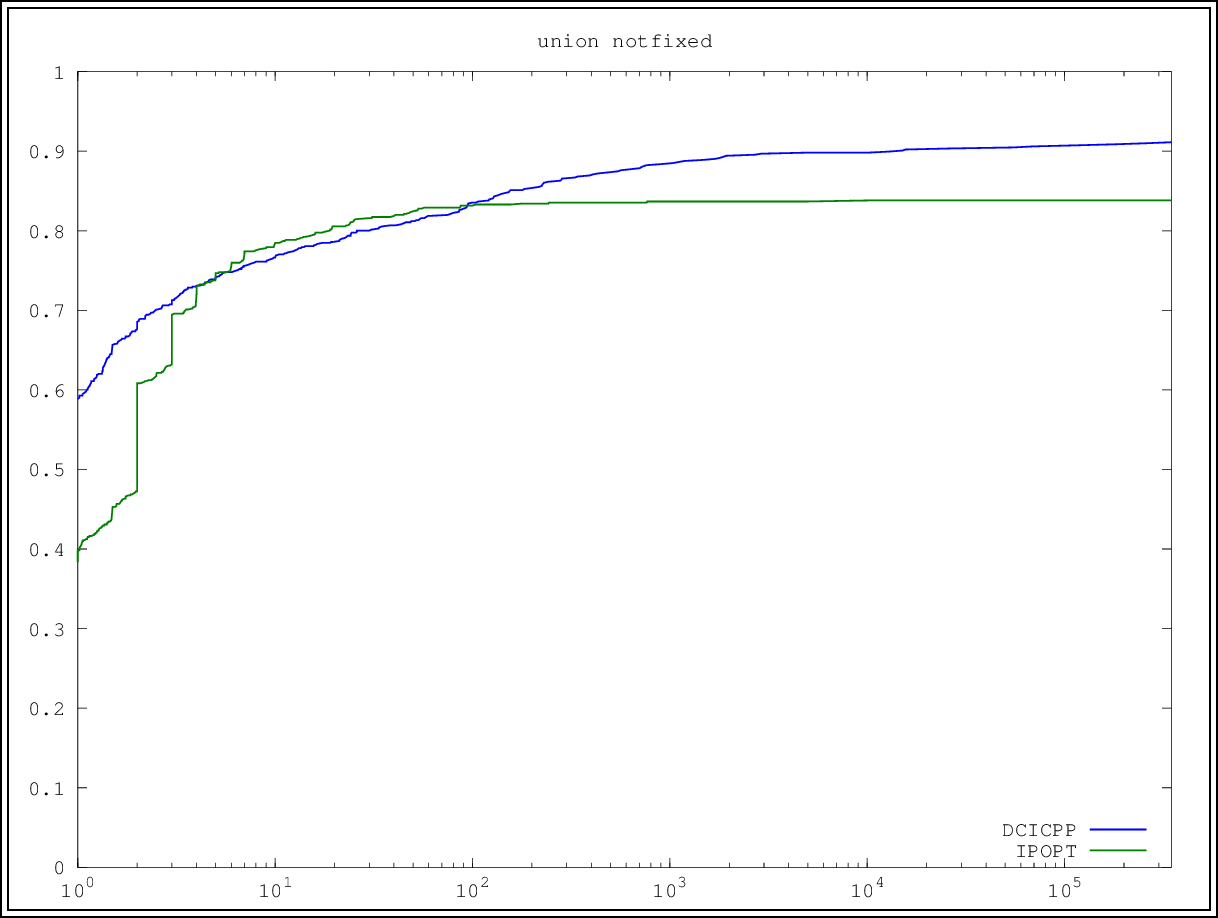
\includegraphics[width=0.8\textwidth]{union_notfixed_strict.png}
\caption{767 problemas pequenos do CUTEr}
\label{fig:small-all}
\end{figure}
Essas comparações indicam que o algoritmo é mais eficiente
que o IPOPT, numa boa quantidade dos problemas. No entanto,
o IPOPT é mais robusto, conseguindo resolver uma quantidade
maior que problemas. Acreditamos que existe espaço para
melhoria no algoritmo, e que é possível alcançar uma boa
porcentagem de convergência.

A Tabela \ref{tab:small} mostra os testes pequenos do CUTEr.
O resultado {\bf Convergiu} indica que o algoritmo convergiu para um ponto
estacionário.
O resultado {\bf Máximo de Iterações} indica que o algoritmo não convergiu no
máximo de iterações.
O resultado {\bf Máximo de Restaurações} indica que o algoritmo normal não
conseguiu encontrar um ponto dentro do cilindro menor no número dado de
iterações.
O resultado {\bf $\rhomax$ pequeno} indica que o cilindro ficou muito
pequeno. 
O resultado {\bf Máximo de tempo} indica que o algoritmo não convergiu no tempo
de execução permitido.
O resultado {\bf Estacionário da Inviabilidade} indica que o algoritmo normal
parou em um ponto estacionário para o problema normal.
O resultado {\bf Ilimitado} indica que a norma do iterando ficou muito grande.
O resultado {\bf Outras falhas} é um conjunto de falhas
específicas para cada problema. Os outros resultados são
auto-explicativos.

\begin{table}[!ht]
\centering
\small
\begin{tabular}{|c||c|c|} \hline
\multirow{2}{*}{\bf Saída do Algoritmo} &
\multicolumn{2}{|c|}{\bf Total} \\ \cline{2-3}
& {\bf \No} & {\bf \%}
\\ \hline
{\bf  Convergiu  } 
& 698  &  91.00   \\ \hline
{\bf  Máximo de Iterações } 
&   5  &   0.65   \\ \hline
{\bf  Máximo de Restaurações } 
&  12  &   1.56   \\ \hline
{\bf  $\rhomax$ pequeno  } 
&  21  &   2.74   \\ \hline
{\bf  Máximo de tempo  } 
&  17  &   2.22   \\ \hline
{\bf  Estacionário da Inviabilidade  } 
&   7  &   0.91   \\ \hline
{\bf  Ilimitado  } 
&   5  &   0.65   \\ \hline
{\bf  Outras Falhas  } 
&   2  &   0.26   \\ \hline
{\bf  Total  } 
& 767  & 100.00   \\ \hline
\end{tabular}
\caption{ Resultados do algoritmo }
\label{tab:small}
\end{table}

Planejamos estudar em detalhes os motivos pelos quais o
DCICPP não converge para os outros problemas, separando-os
em classes diferentes e analisando separadamente cada
classe. Também queremos procurar outros métodos para 
resolver os subproblemas e avaliar se as Jacobianas
mal condicionadas são responsáveis pela falha de alguns
problemas. 
Aproveitaremos para poder melhorar a usabilidade
do algoritmo, e incluir a possibilidade de variáveis
fixas. Dessa maneira, teremos um algoritmo mais competitivo.

\section{Cronograma}

\begin{itemize}
 \item {\bf  Dezembro de 2013 - Junho de 2013}
   \begin{itemize}
     \item Separação e estudo dos problemas com falha do algoritmo.
     \item Tratamento das variáveis fixas. 
   \end{itemize}
 \item {\bf  Julho de 2013 - Novembro de 2014}
   \begin{itemize}
     \item Implementação de outras estratégias de resolução dos subproblemas.
     \item Estudo das Jacobianas mal condicionadas.
     \item Limpeza do código.
   \end{itemize}
\end{itemize}

\bibliographystyle{plainnat}
\bibliography{relbib}

\end{document}
